\documentclass{beamer}
\usepackage{ucs}
\usepackage[utf8]{inputenc}
\usepackage{ngerman}
\usepackage[ngerman]{babel}
\usepackage{floatflt}
\usepackage{listings}
\usepackage{minted}
\definecolor{lightgray}{rgb}{.95,.95,.95}
\definecolor{darkblue}{rgb}{0,0,.6}
\definecolor{darkred}{rgb}{.6,0,0}
\definecolor{darkgreen}{rgb}{0,.6,0}
\definecolor{red}{rgb}{.98,0,0}
\lstloadlanguages{C++}
\lstset{%
	language=C++,
	basicstyle=\footnotesize\ttfamily,
	commentstyle=\color{darkgreen},%\itshape
	keywordstyle=\bfseries\color{darkblue},
	stringstyle=\color{darkred},
	showspaces=false,
	showtabs=false,
	columns=fixed,
	numbers=left,
	frame=none,
	numberstyle=\tiny,
	breaklines=true,
%	backgroundcolor=\color{lightgray},
	showstringspaces=false,
	xleftmargin=1cm
}%

\usepackage{beamerthemesplit}

\title{LIFI Live Feedback}
\subtitle{Meilenstein 3}
\author{Gruppe 5 (Paul Walger, Sebastian Götte)}
\institute{TU Berlin}
\date{17. Juli 2015}
\usetheme{Copenhagen}
\usecolortheme{crane}

\begin{document}

\frame{\titlepage}

\section{Backend}
\begin{frame}
    \frametitle{Datenmodell}
    \begin{center}
        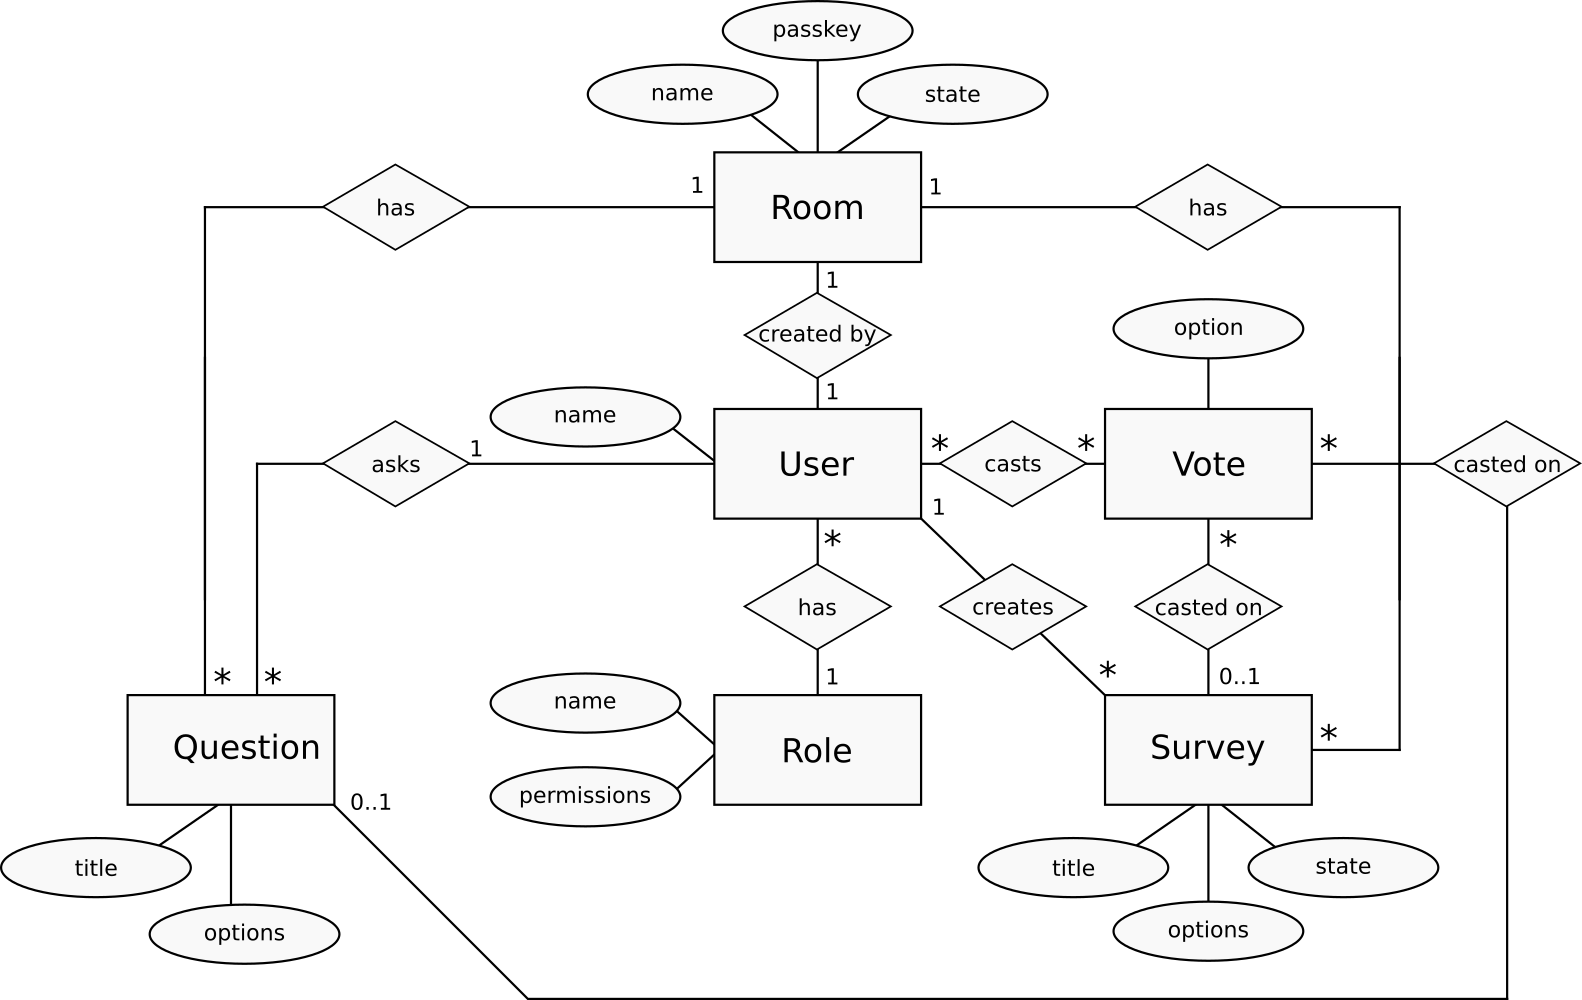
\includegraphics[width=10cm]{../MS1/diagrams/er/er_diagram.png}
    \end{center}
\end{frame}
% Abstimmungssicherheitsgedöns
\begin{frame}
    \begin{center}
        
\includegraphics[width=10cm]{diagrams/roles-1.png}
    \end{center}
\end{frame}
\begin{frame}
    \frametitle{Rollen}
    \begin{tabular}{lll}
        \textbf{Teilnehmer}&\textbf{Veranstalter}&\textbf{Administrator}\\
        \texttt{view\_index}&       \texttt{manage\_lecture}&  \texttt{create\_account}\\
        \texttt{view\_room}&        \texttt{create\_survey}&   \texttt{delete\_account}\\
        \texttt{create\_question}&  \texttt{create\_room}&     \texttt{assign\_role}\\
        \texttt{join\_lecture}&     \texttt{view\_tempo}&      \texttt{create\_role}\\
        \texttt{vote\_tempo}&       \texttt{close\_survey}&    \texttt{edit\_role}\\
        \texttt{vote\_question}&    \texttt{delete\_question}& \texttt{delete\_role}\\
        \texttt{vote\_survey}&      \texttt{delete\_survey}&   \texttt{list\_roles}\\
        \texttt{list\_permissions}& \texttt{}&                 \texttt{list\_users}
    \end{tabular}
\end{frame}
\section{Eingesetzte Technologien}
\begin{frame}
    \frametitle{Serversoftware}
    \begin{itemize}
        \item Postgresql
        \item Python 3
        \item nginx
    \end{itemize}
\end{frame}
\begin{frame}
    \frametitle{Python-Server}
    \begin{itemize}
        \item Flask (HTTP-Microframework)
        \item SQLAlchemy (ORM)
    \end{itemize}
\end{frame}
\newminted{python3}{breaklines}
\newminted{rst}{breaklines}
\begin{frame}[fragile]
    \frametitle{Authentifizierung}
    \begin{block}{\texttt{auth}-Decorator}
    \begin{python3code}
@app.route('/api/r/<room_name>')
@auth
@room
def view_room(room):
    return jsonify(name=room.name,
            questions=[ q.as_dict() for q in room.questions ],
            surveys=[ sv.as_dict() for sv in room.surveys ],
            user_is_lecturer=(room.creator == request.user))
    \end{python3code}
    \end{block}
\end{frame}
\begin{frame}[fragile]
    \frametitle{Unit-Testing}
    \begin{block}{\texttt{test\_for}-Decorator}
    \begin{python3code}
@test_for('list_rooms', """
:HTTP method:   GET
:Response JSON: ``{"rooms": ["some_room", "another_room"]}`` """)
def testListRooms(self):
    with testserver() as url:
        cred = self.login(url, 'user1')
        r = rq.get(url+'list_rooms', cookies=cred)
        self.json(r, {'rooms': {'test_room_access', 'test_room_deny'}})
    \end{python3code}
    \end{block}
\end{frame}
\begin{frame}[fragile]
    \frametitle{Api-Dokumentation}
    \begin{block}{Automatische Dokumentation in \texttt{rst}, \texttt{tex} und \texttt{pdf}}
    \begin{rstcode}
list_rooms
==========
:Routes:
    ``/api/list_rooms``
:HTTP method:   GET
:Response JSON: ``{"rooms": ["some_room", "another_room"]}``
    \end{rstcode}
    \end{block}
\end{frame}
\section{Web-Frontend}
% Screenshots!
\section{Android-Frontend}
% Screenshots!
% Unterschiede zum Web-Frontend
\section{Entwicklung und Deployment}
% Entwicklung mit SVN/GIT
% Deployment via Ansible
% Testen mit Vagrant
% Lokales Testen mit Virtualenv und Gulp
\section{Demo}
\end{document}
